\section{FEM Overview}
\frame{\tableofcontents[currentsection,hideothersubsections]}

\lstset{language=bash,
  basicstyle=\ttfamily,
  keywordstyle=\ttfamily,
  showtabs=true,
%  showspaces=true,
  tabsize=3,
  tab=\hrulefill}
%%%%%%%%%%%%%%%%%%%%%%%%%%%%%%%%%%%%%%%%%%%%%%%%%%%%%%%%%%%%%%%%%%%%%%
%%%%%%%%%%%%%%%%%%%%%%%%%%%%%%%%%%%%%%%%%%%%%%%%%%%%%%%%%%%%%%%%%%%%%%
\subsection{Finite elements}

%%%%%%%%%%%%%%%%%%%%%%%%%%%%%%%%%%%%%%%%%%%%%%%%%%%%%%%%%%%%%%%%%%%%%%
\begin{frame}
  \frametitle{Local finite element spaces}
  \begin{enumerate}
  \item Choose a finite dimensional space $\mathcal P_K$ on each cell $K$
    \begin{itemize}
    \item usually polynomials, sometimes trigonometrics
    \end{itemize}
  \item Define node functionals $n_{K,i}$
    \begin{itemize}
    \item Interpolation points or integral moments
    \item $n_{K,i}$ can be associated with cells, faces, edges,
      vertices
    \item $n_{K,i}(v)$ selects a basis $\{\psi_j\}$ for $\mathcal P_K$ by
      \begin{gather*}
        n_{K,i}(\psi_j) = \delta_{ij}
      \end{gather*}
    \end{itemize}
  \item Identifying nodes between cells creates continuity
  \end{enumerate}
  \begin{center}
    \includegraphics[height=.4\textheight]{graph/concatenation.tikz}
  \end{center}
\end{frame}

\begin{frame}
  \frametitle{Example: $Q_2$}
  \begin{columns}
    \begin{column}{.35\textwidth}
      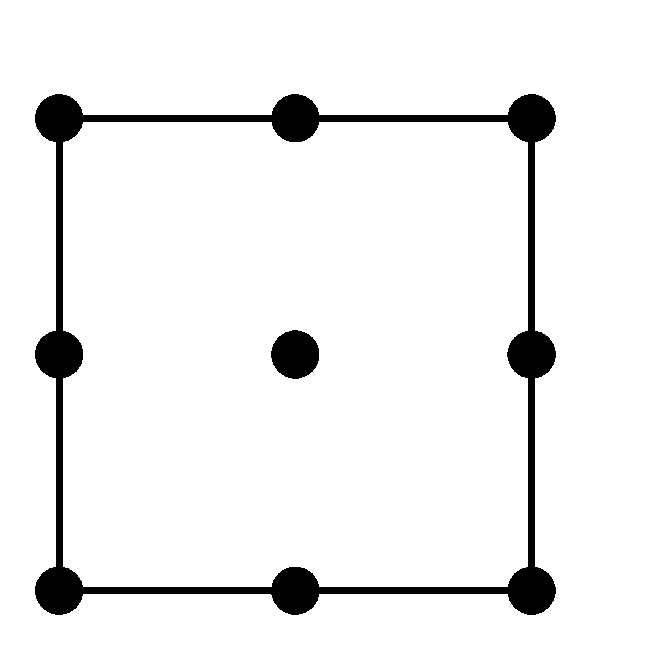
\includegraphics[width=\textwidth]{graph/nodes_q2}
    \end{column}
    \begin{column}{.65\textwidth}
      \begin{itemize}
      \item Tensor product polynomials
        \begin{gather*}
          Q_k = \bigl\{p(x)q(y)\big|
          p,q\in P_2\bigr\}
        \end{gather*}
      \item Quadrature for node functionals
        \begin{itemize}
        \item Others possible, e.g. moments
        \end{itemize}
      \end{itemize}
    \end{column}
  \end{columns}
\end{frame}

\begin{frame}
  \frametitle{Example: $Q_2$ shape functions}
  \begin{center}
    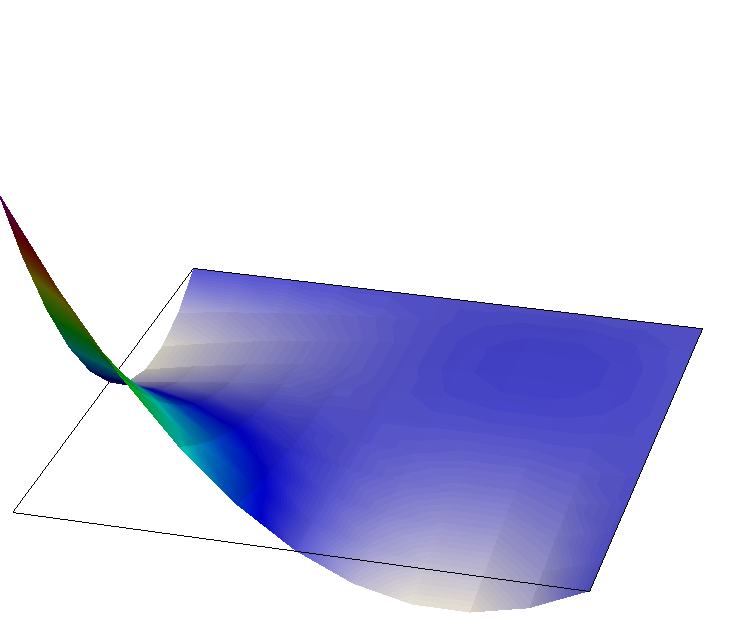
\includegraphics[height=.3\textheight]{graph/shape0}
    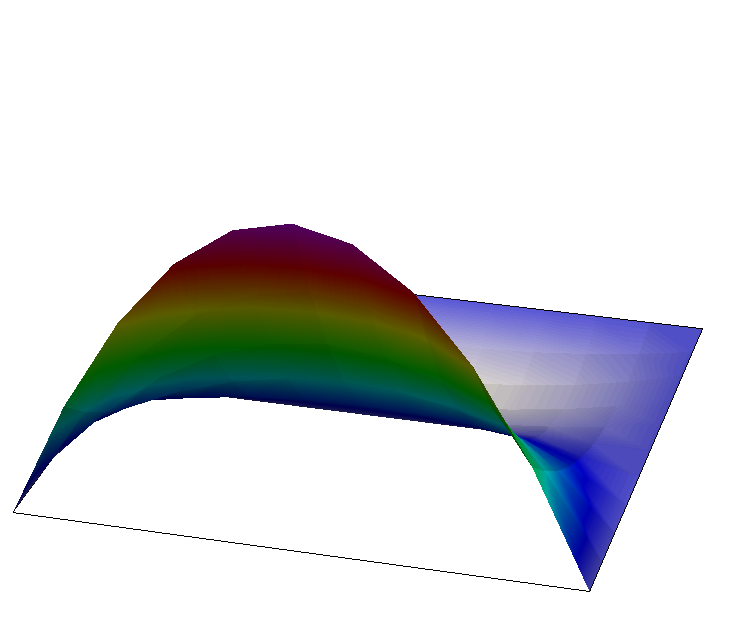
\includegraphics[height=.3\textheight]{graph/shape1}
    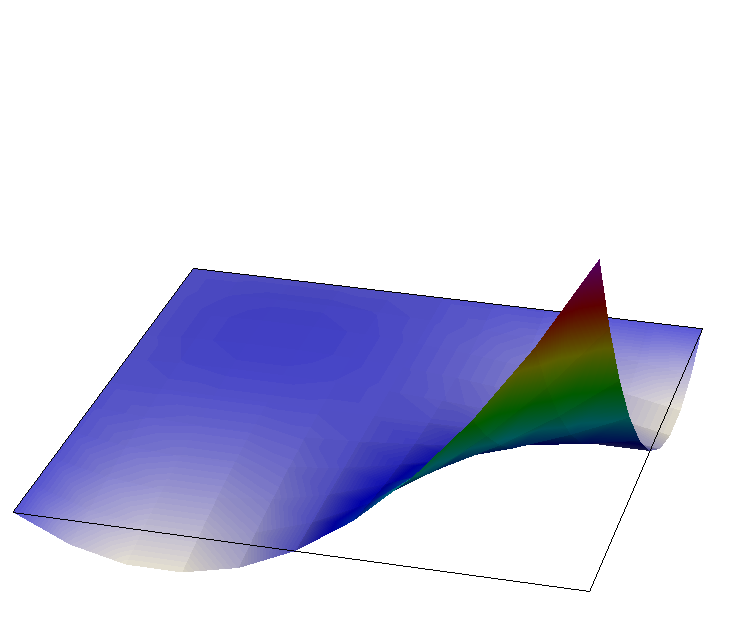
\includegraphics[height=.3\textheight]{graph/shape2}

    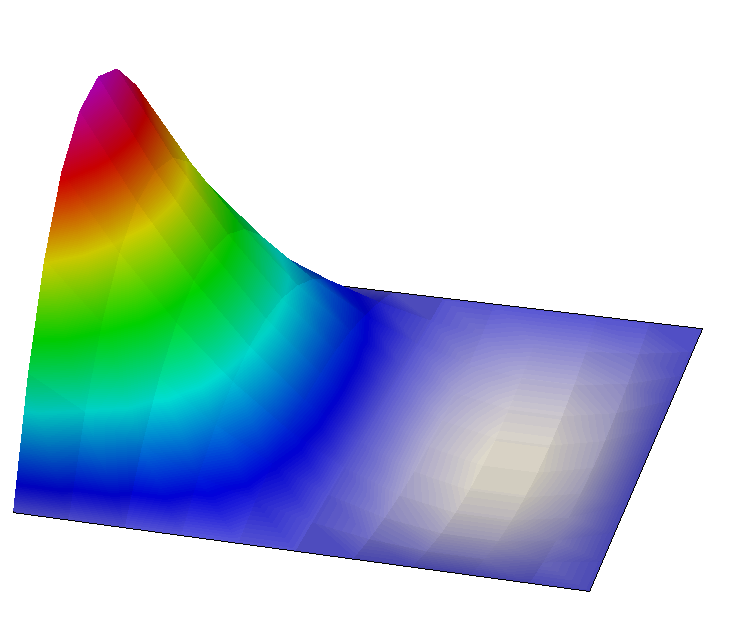
\includegraphics[height=.3\textheight]{graph/shape3}
    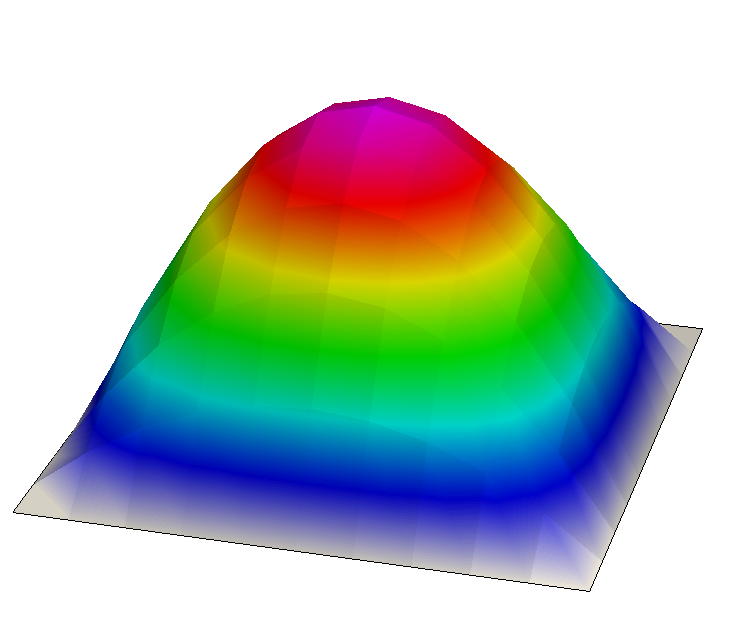
\includegraphics[height=.3\textheight]{graph/shape4}
    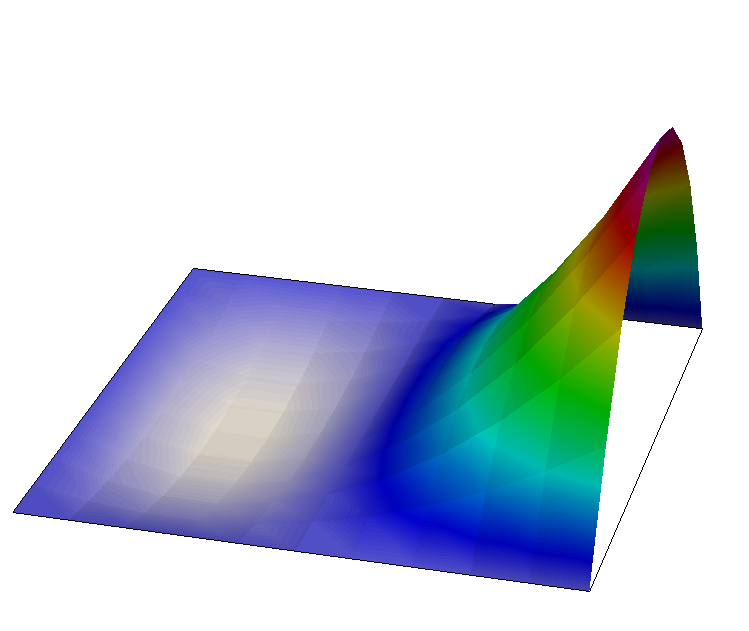
\includegraphics[height=.3\textheight]{graph/shape5}

    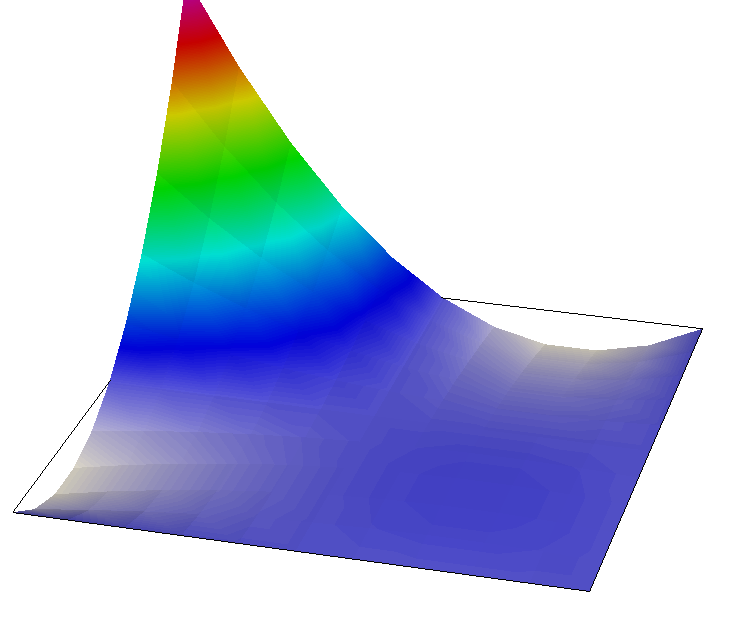
\includegraphics[height=.3\textheight]{graph/shape6}
    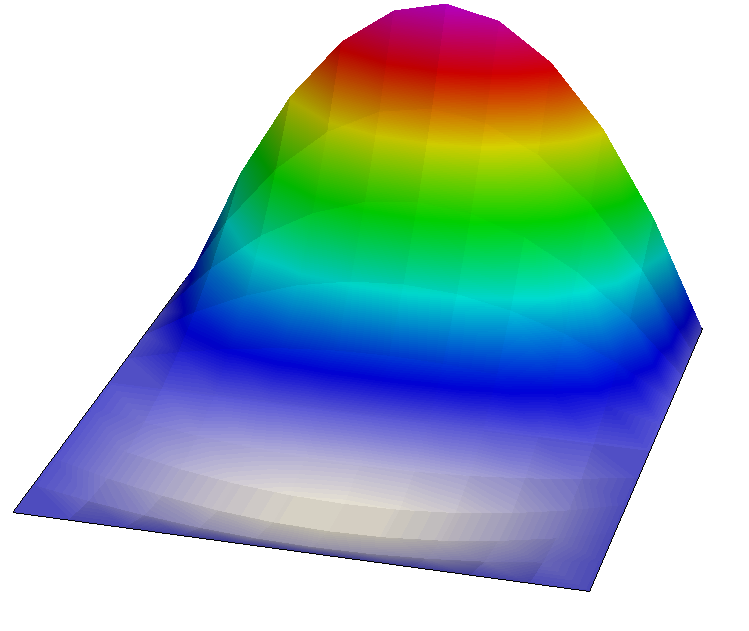
\includegraphics[height=.3\textheight]{graph/shape7}
    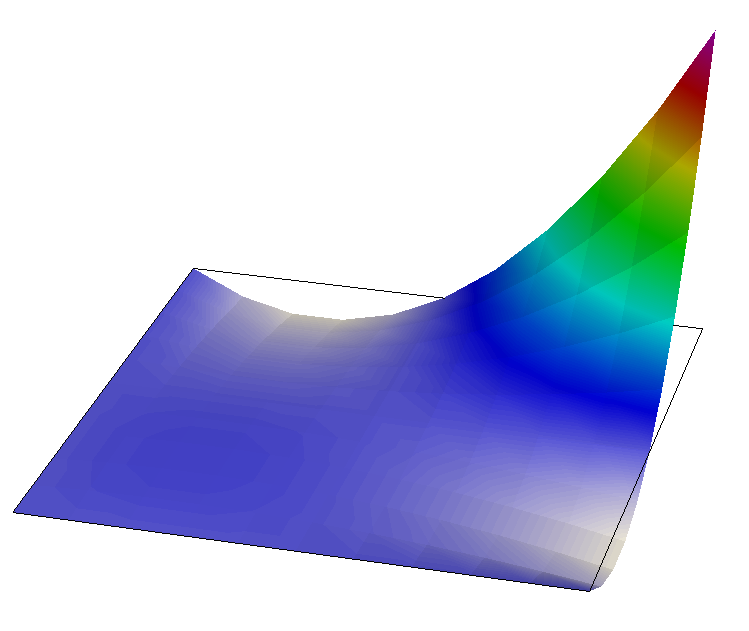
\includegraphics[height=.3\textheight]{graph/shape8}
  \end{center}
\end{frame}

%%%%%%%%%%%%%%%%%%%%%%%%%%%%%%%%%%%%%%%%%%%%%%%%%%%%%%%%%%%%%%%%%%%%%%
\begin{frame}
  \frametitle{Global finite element spaces}
  \begin{itemize}
  \item Throw a mesh over the domain $\Omega$
  \item Concatenate the spaces $P_K$ to obtain discrete space $V_h$
  \item Eliminate identified degrees of freedom and count globally
  \item ``Glued'' shape functions become basis functions $\phi_i$
    \begin{itemize}
    \item $i$ is a ``global'' index unique for the whole mesh
    \end{itemize}
  \end{itemize}
\end{frame}

% TODO: Q2 basis functions

\begin{frame}
  \frametitle{Example: $Q_2$ continuous basis (selection)}
  \begin{center}
    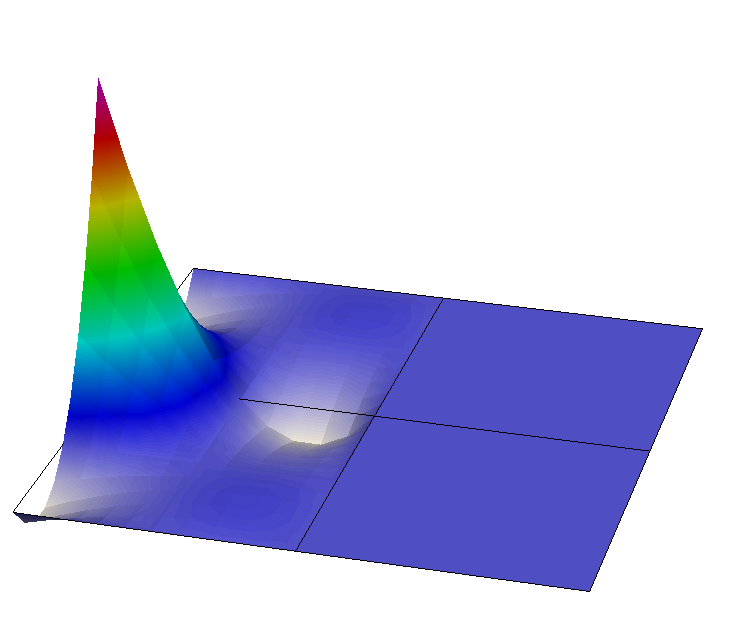
\includegraphics[height=.27\textheight]{graph/cgbasis1-02}
    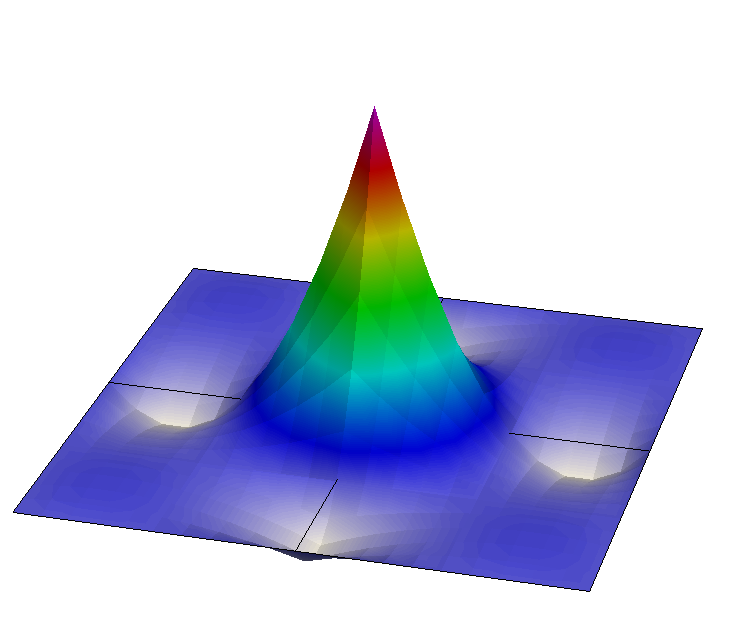
\includegraphics[height=.27\textheight]{graph/cgbasis1-03}
    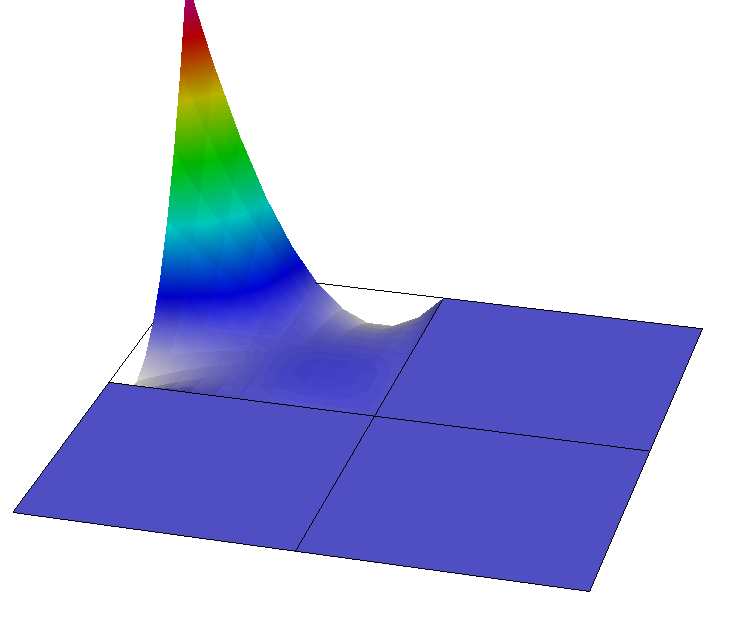
\includegraphics[height=.27\textheight]{graph/cgbasis1-15}
    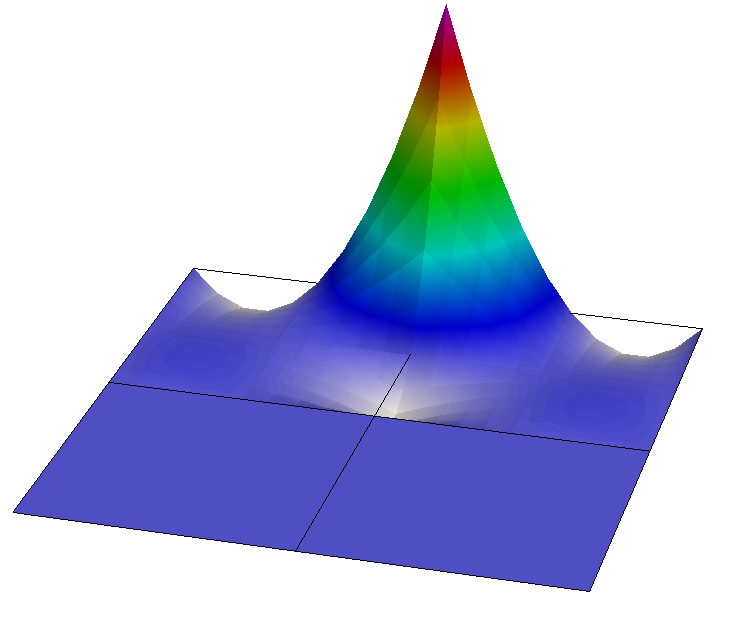
\includegraphics[height=.27\textheight]{graph/cgbasis1-16}

    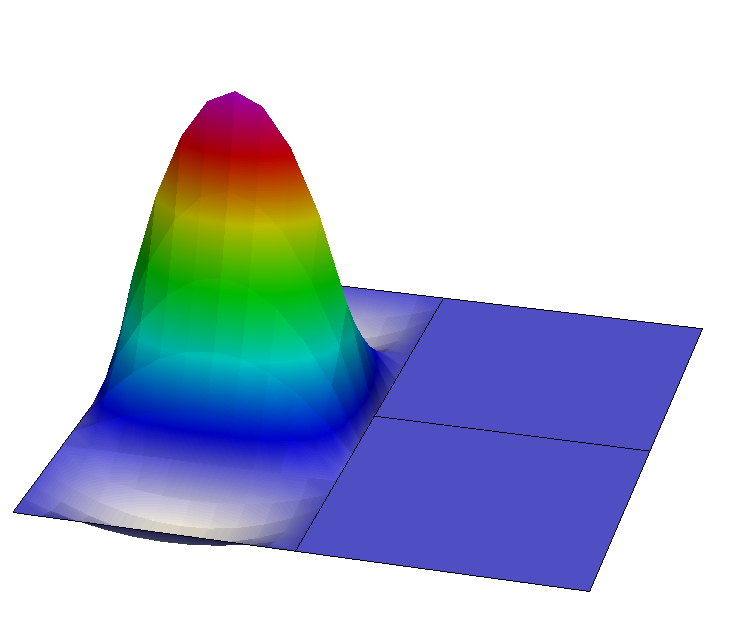
\includegraphics[height=.27\textheight]{graph/cgbasis1-07}
    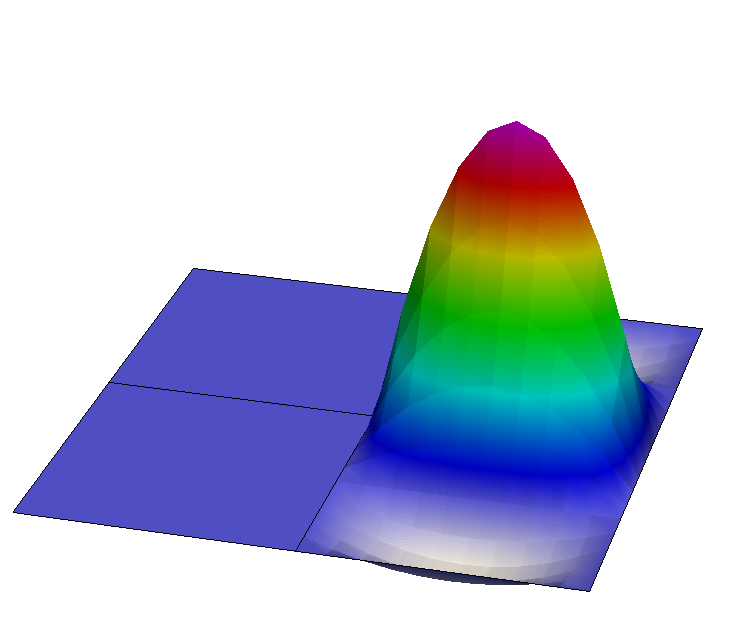
\includegraphics[height=.27\textheight]{graph/cgbasis1-13}
    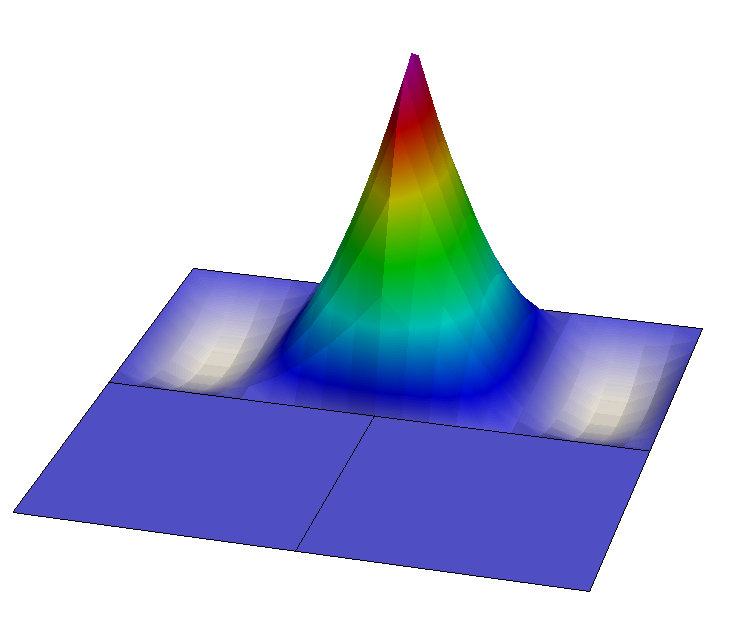
\includegraphics[height=.27\textheight]{graph/cgbasis1-18}
    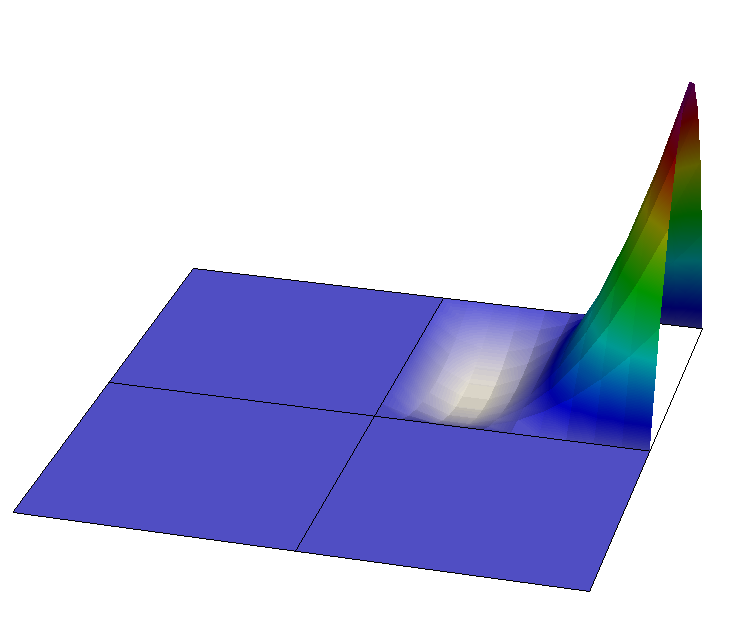
\includegraphics[height=.27\textheight]{graph/cgbasis1-22}

    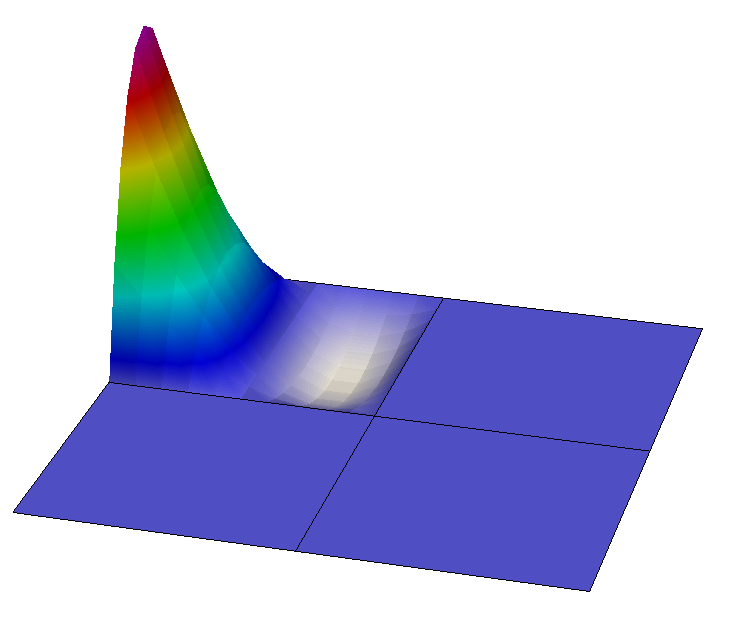
\includegraphics[height=.27\textheight]{graph/cgbasis1-17}
    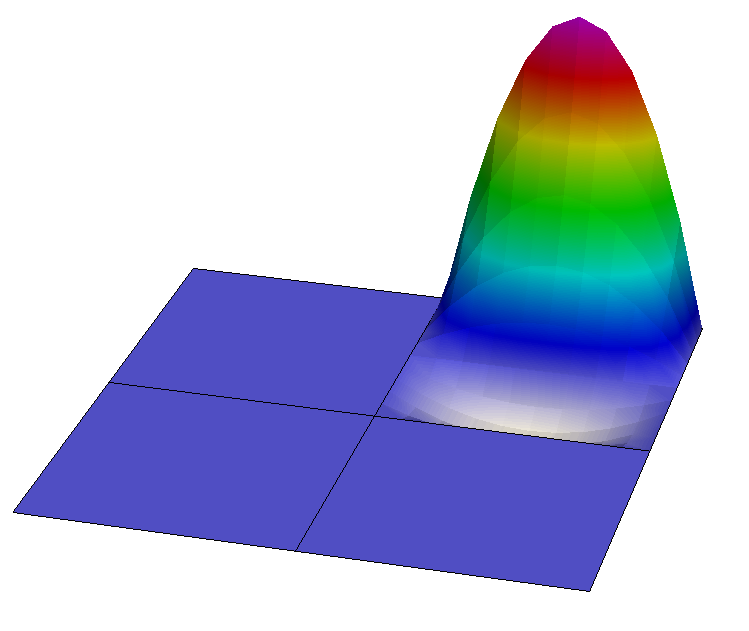
\includegraphics[height=.27\textheight]{graph/cgbasis1-23}
    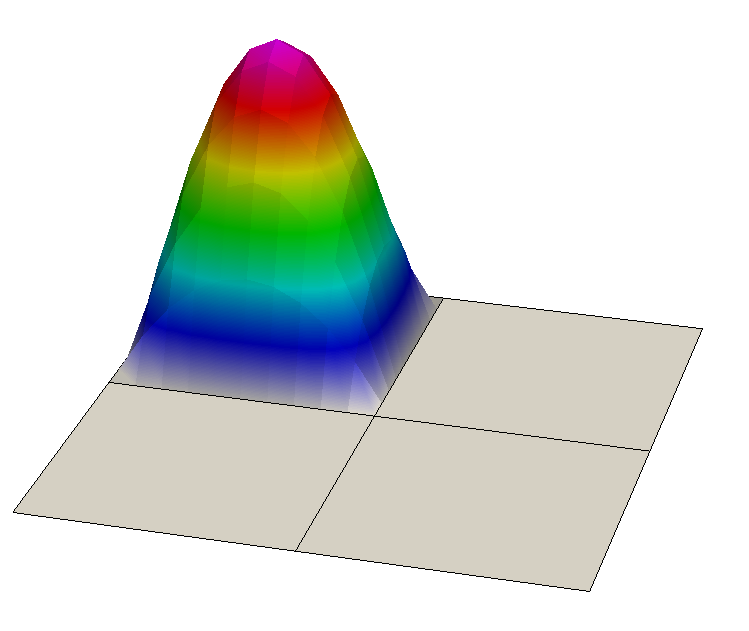
\includegraphics[height=.27\textheight]{graph/cgbasis1-20}
    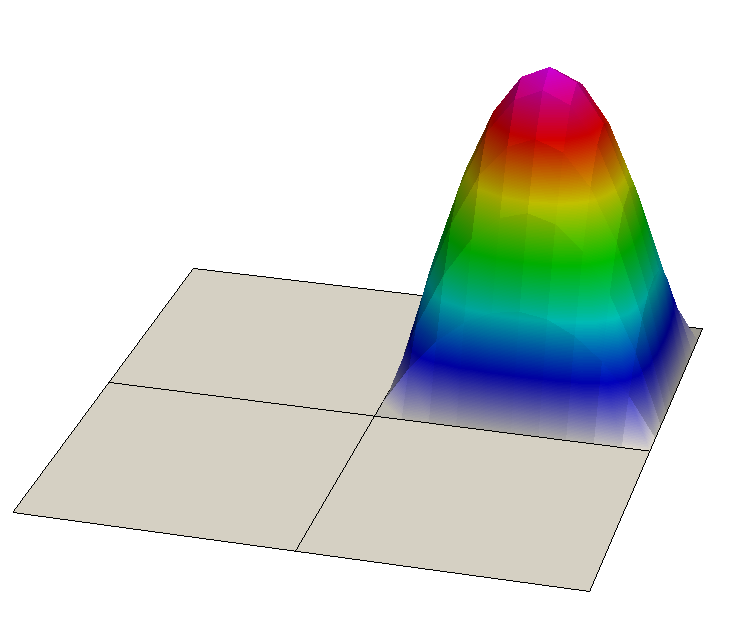
\includegraphics[height=.27\textheight]{graph/cgbasis1-24}
  \end{center}
\end{frame}

\begin{frame}
  \frametitle{Example: $Q_2$ discontinuous basis (selection)}
  \begin{center}
    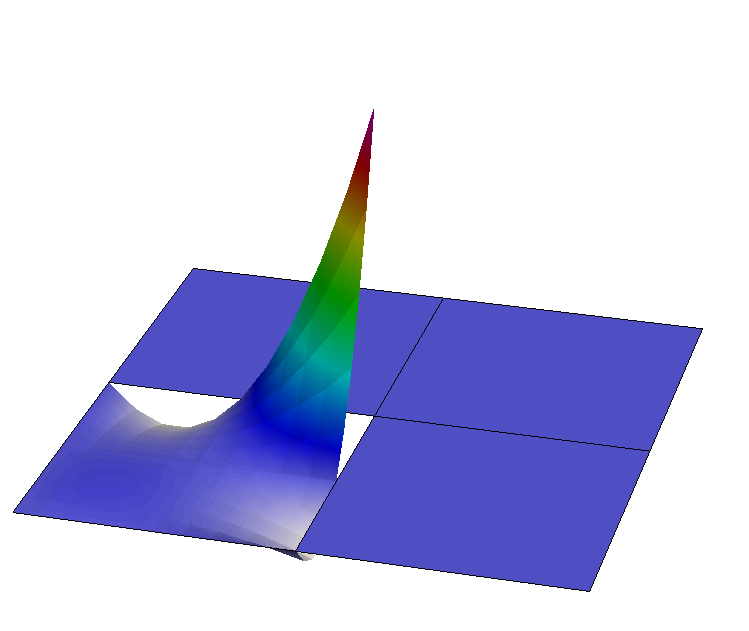
\includegraphics[height=.27\textheight]{graph/dgbasis1-08}
    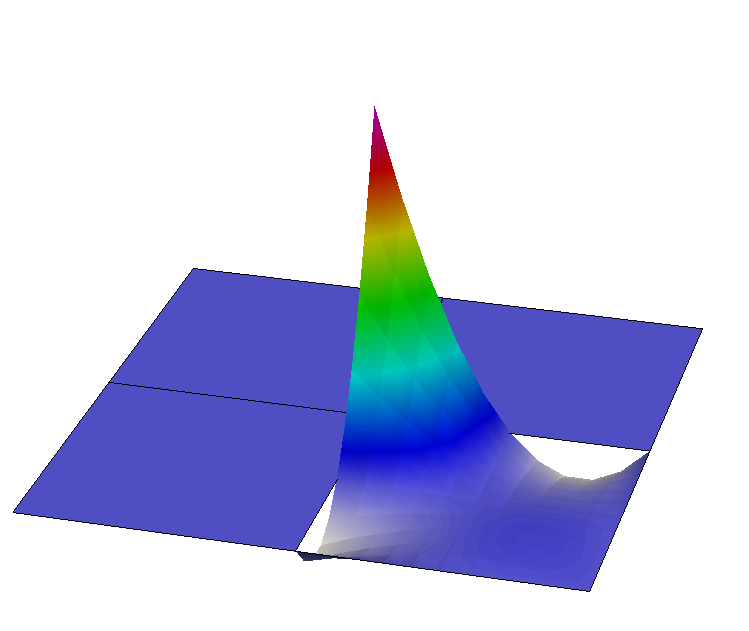
\includegraphics[height=.27\textheight]{graph/dgbasis1-15}
    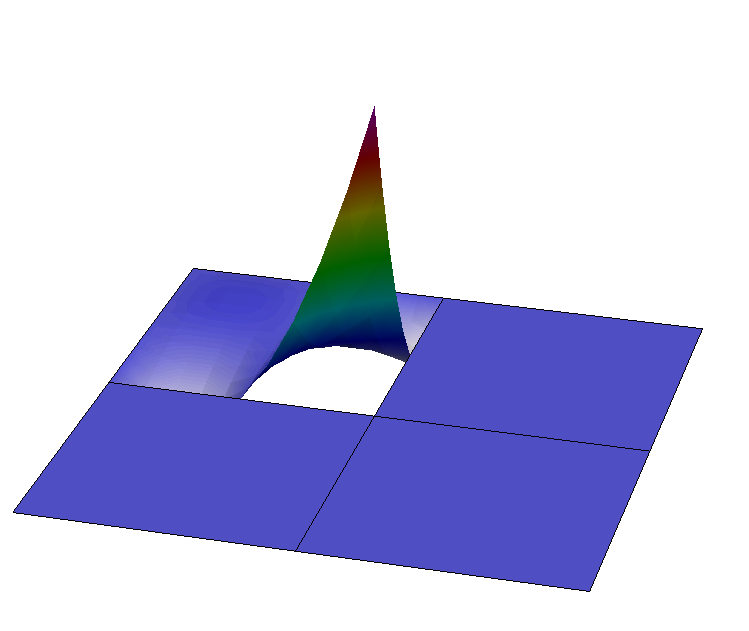
\includegraphics[height=.27\textheight]{graph/dgbasis1-20}
    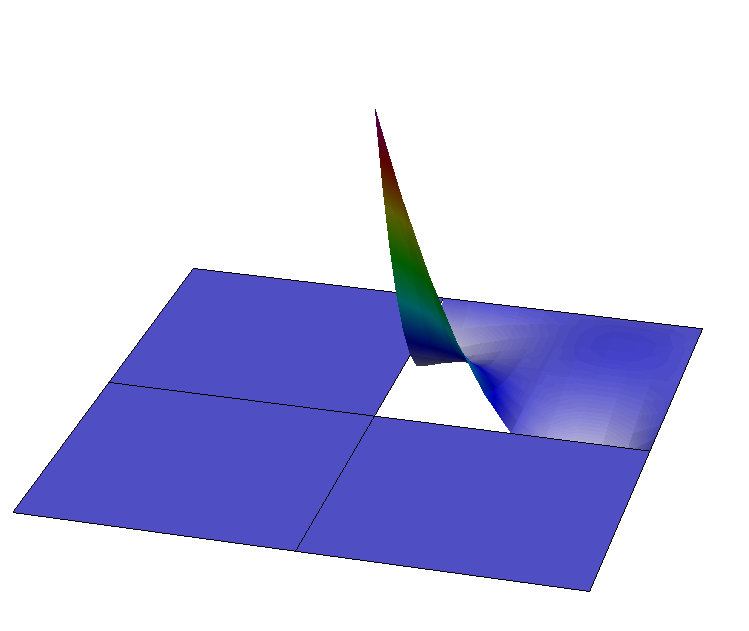
\includegraphics[height=.27\textheight]{graph/dgbasis1-27}

    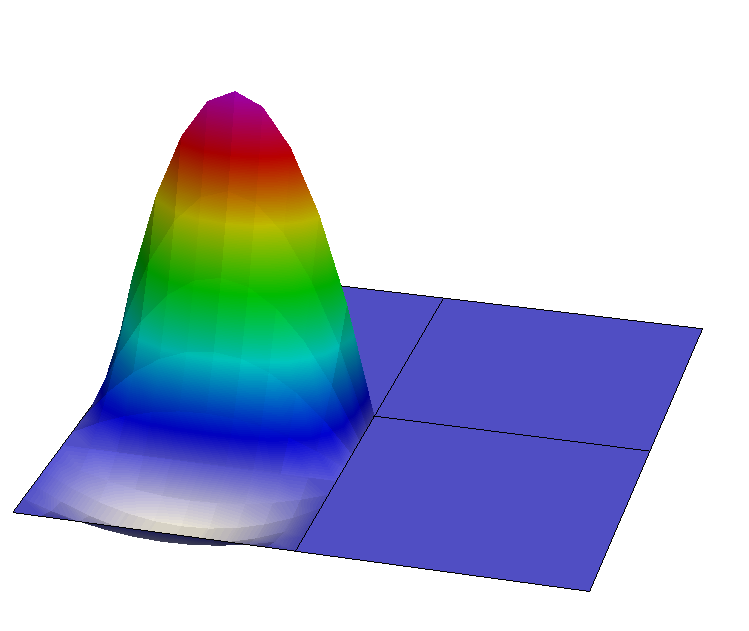
\includegraphics[height=.27\textheight]{graph/dgbasis1-07}
    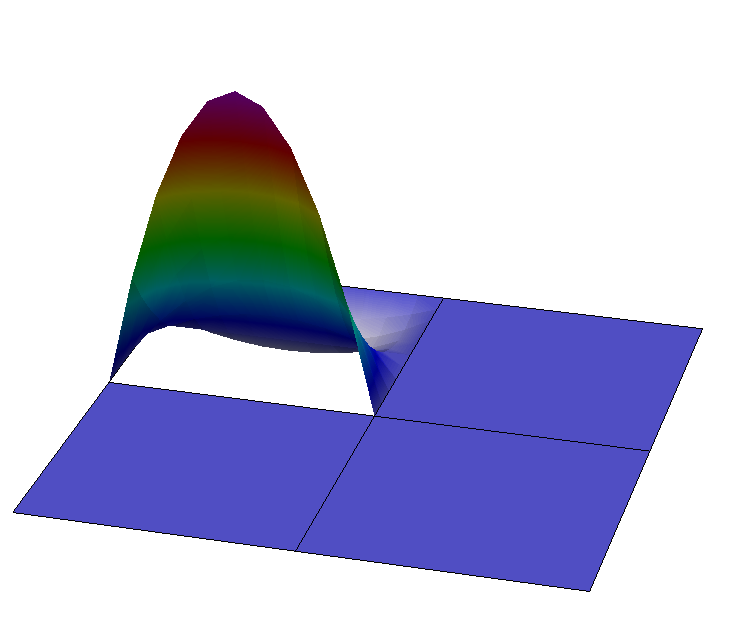
\includegraphics[height=.27\textheight]{graph/dgbasis1-19}
    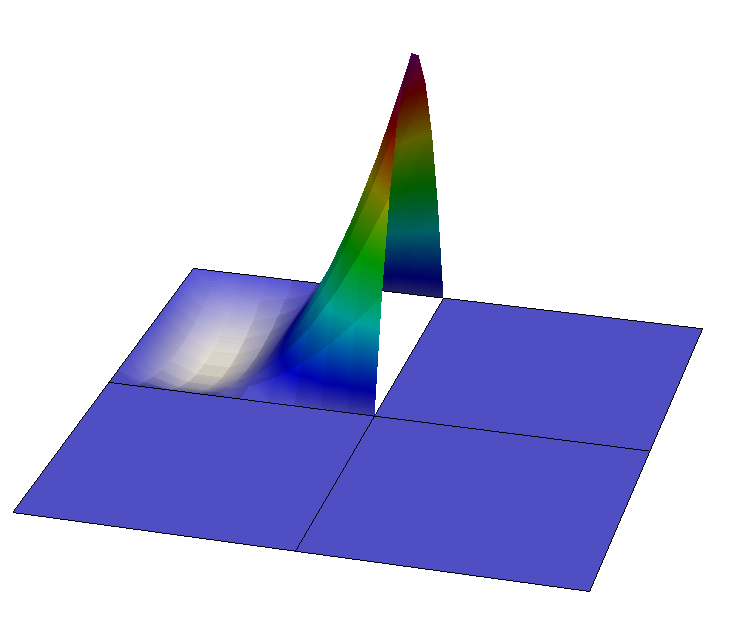
\includegraphics[height=.27\textheight]{graph/dgbasis1-23}
    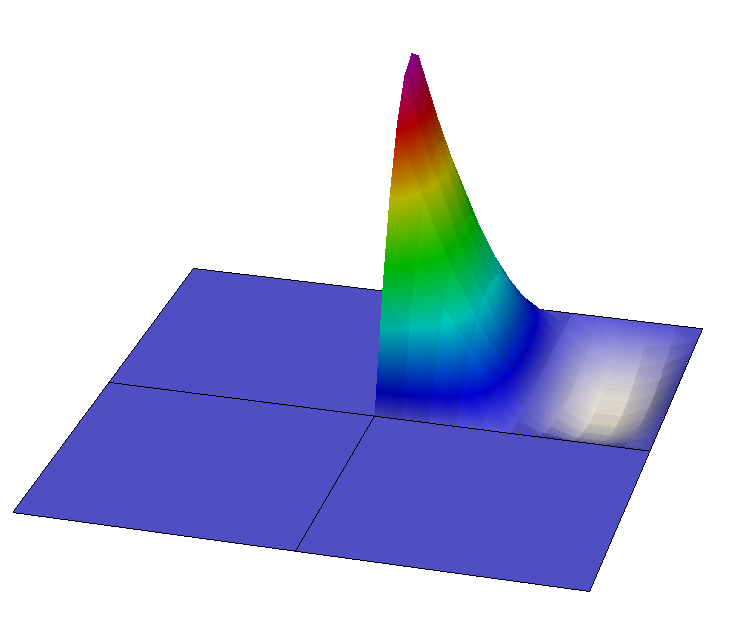
\includegraphics[height=.27\textheight]{graph/dgbasis1-30}

    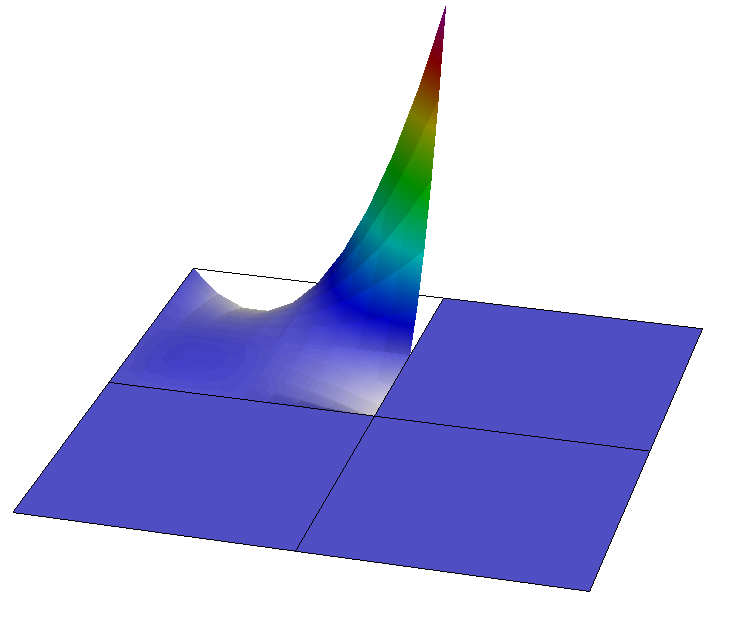
\includegraphics[height=.27\textheight]{graph/dgbasis1-26}
    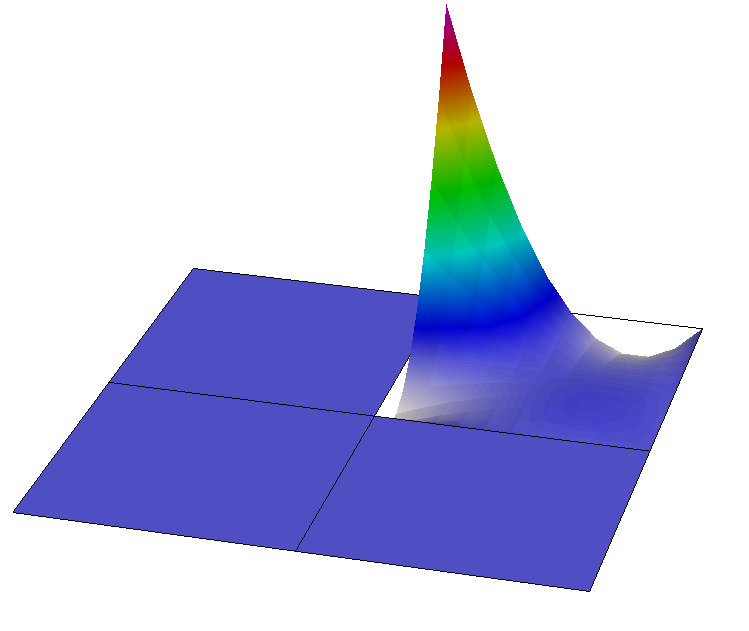
\includegraphics[height=.27\textheight]{graph/dgbasis1-33}
    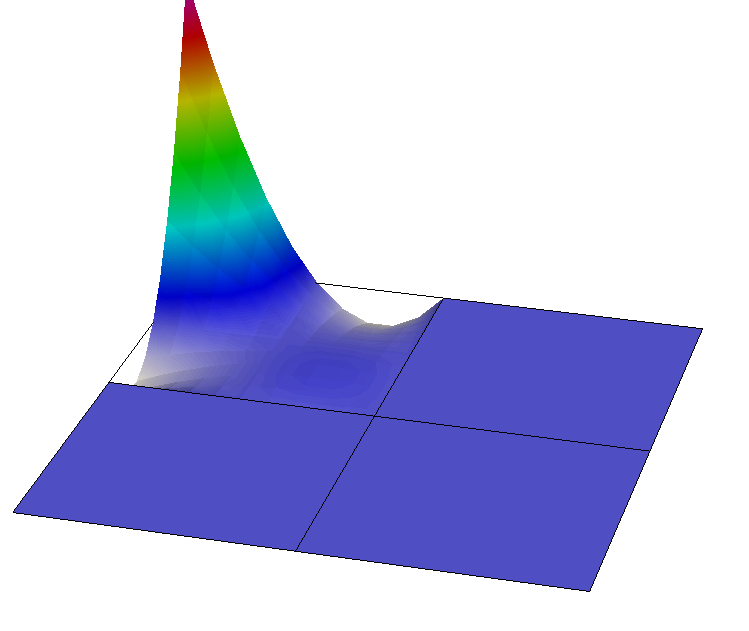
\includegraphics[height=.27\textheight]{graph/dgbasis1-24}
    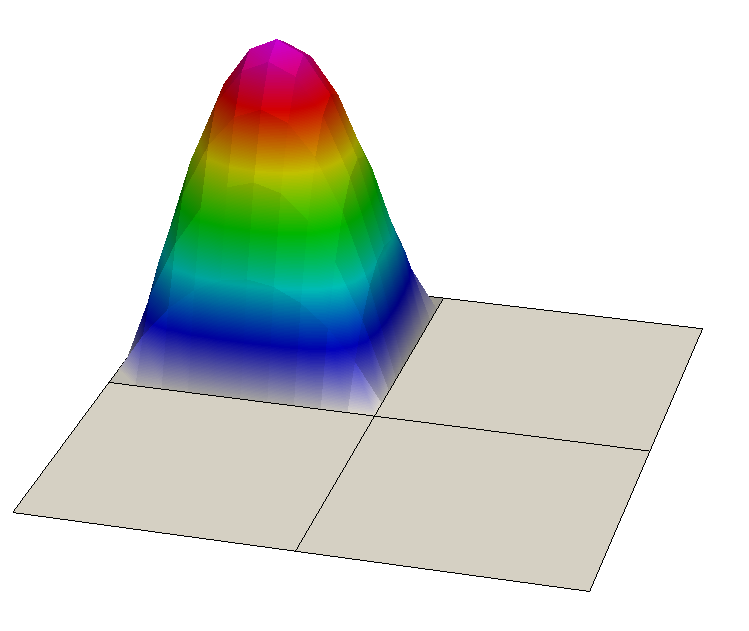
\includegraphics[height=.27\textheight]{graph/dgbasis1-22}
  \end{center}
\end{frame}

%%%%%%%%%%%%%%%%%%%%%%%%%%%%%%%%%%%%%%%%%%%%%%%%%%%%%%%%%%%%%%%%%%%%%% 
\begin{frame}
  \frametitle{Finite Element Spaces in deal.II}
  \begin{itemize}
  \item Meshes are handled by \lstinline!Triangulation<dim,sdim>!
  \item Classes derived from \lstinline!FiniteElement<dim,sdim>!
    define ``shape function space'' and ``node values''
  \item \lstinline!DoFHandler<dim,sdim>! administers the ``global
    finite element space''
  \end{itemize}
  \begin{block}{}
    \lstinputlisting{code/generic_setup.cc}
  \end{block}
\end{frame}

%%%%%%%%%%%%%%%%%%%%%%%%%%%%%%%%%%%%%%%%%%%%%%%%%%%%%%%%%%%%%%%%%%%%%%
%%%%%%%%%%%%%%%%%%%%%%%%%%%%%%%%%%%%%%%%%%%%%%%%%%%%%%%%%%%%%%%%%%%%%%
\subsection{Weak formulation}

%%%%%%%%%%%%%%%%%%%%%%%%%%%%%%%%%%%%%%%%%%%%%%%%%%%%%%%%%%%%%%%%%%%%%%
\begin{frame}
  \frametitle{A model problem}
  \begin{itemize}
  \item Poisson problem with Dirichlet boundary conditions
    \begin{gather*}
      -\Delta u = f \text{ in }\Omega,\qquad u=0 \text{ on }\partial\Omega.
    \end{gather*}
  \item Weak formulation: find $u\in V = H^1_0(\Omega)$ such that
    \begin{gather*}
      \int_\Omega \nabla u\cdot \nabla v \,dx
      =
      \int_\Omega fv\,dx
      \quad\forall v\in V
    \end{gather*}
  \end{itemize}
\end{frame}

%%%%%%%%%%%%%%%%%%%%%%%%%%%%%%%%%%%%%%%%%%%%%%%%%%%%%%%%%%%%%%%%%%%%%%
\begin{frame}
  \frametitle{Weak form for FEM}
  \begin{itemize}
  \item Find $u\in V_h$ such that
    \begin{gather*}
      \int_\Omega \nabla u\cdot \nabla v \,dx
      =
      \int_\Omega fv\,dx
      \quad\forall v\in V_h
    \end{gather*}
  \item The weak formulation
    \begin{gather*}
      a(u,v) = f(v)
    \end{gather*}
  \item The discrete problem (linear algebra)
    \begin{gather*}
      \only<2->{v^T} Au =  \only<2->{v^T}f
    \end{gather*}
  \end{itemize}
  \pause
  \begin{block}{Warning!!!}
    The order of trial and test space is reverted!
    \begin{gather*}
      a_{\red ij} = %\sum_{K \in \mathbb T_h}
      a(\phi_j, \phi_i)
    \end{gather*}
  \end{block}
\end{frame}

\begin{frame}
  \frametitle{Implementation of the integrals}
  \begin{itemize}
  \item Split the integrals
    \begin{gather*}
      \int_\Omega \bullet \, dx = \sum_{K \in \T_h}\int_K \bullet \; dx
    \end{gather*}
  \item Only small number of shape functions get integrated
    \begin{itemize}
    \item Complexity linear in number of cells!
    \end{itemize}
  \item Local integrals are simple and computed by quadrature
    \begin{gather*}
      a_{ij}^K = \int_K \nabla \psi_j \cdot \nabla \psi_i\,d x
    \end{gather*}
  \item Mapping from local to global indices to add cell matrices $A_K$
  \end{itemize}
\end{frame}

%%%%%%%%%%%%%%%%%%%%%%%%%%%%%%%%%%%%%%%%%%%%%%%%%%%%%%%%%%%%%%%%%%%%%%
%%%%%%%%%%%%%%%%%%%%%%%%%%%%%%%%%%%%%%%%%%%%%%%%%%%%%%%%%%%%%%%%%%%%%%
\subsection{Solving the discrete problems}

%%%%%%%%%%%%%%%%%%%%%%%%%%%%%%%%%%%%%%%%%%%%%%%%%%%%%%%%%%%%%%%%%%%%%%
\begin{frame}
  \frametitle{Sparse matrices}
  \begin{itemize}
  \item Matrices from finite element discretizations tend to be large
    \begin{itemize}
    \item $10^6$ to $10^9$ rows are common nowadays
    \item Example: $Q_1$ on a $100^3$ grid in 3D
    \end{itemize}
  \item Only basis functions with common support generate entries
    \begin{itemize}
    \item Only functions on a cell
    \item Very few entries per line
    \item Entries are scattered according to the mesh and numbering
    \end{itemize}
  \end{itemize}
\end{frame}

%%%%%%%%%%%%%%%%%%%%%%%%%%%%%%%%%%%%%%%%%%%%%%%%%%%%%%%%%%%%%%%%%%%%%%
\begin{frame}
  \frametitle{Effort for linear solvers}
  Example: uniform mesh of $100^3$ cells, $10^9$ flops/sec
  \begin{itemize}
  \item<+-> Gauß elimination, $LU$ decomposition
    \only<2->{: 10 years}
    \only<1>{\begin{itemize}
    \item Effort: $n^3/3 + \mathcal O(n^2)$ flops
    \item Example: $100^9/3 = 10^{18}/3 \text{flops} \approx 10^9/3 \text{sec}
      \approx 10^4/3 \text{days} \approx 10  \text{years}$
    \end{itemize}}
  \item<+-> Banded version, skyline solver
    \only<3->{: 8 hours}
    \only<2>{\begin{itemize}
    \item Effort: $n/3 (n^{2/3})^2 + \mathcal O(n^2)
      \approx n^{7/3}$ flops
    \item Example: $100^7/3 = 10^{14}/3 \text{flops}
      \approx 10^5/3 \text{sec}
      \approx 8 \text{hours}$
    \end{itemize}}
  \item<+-> Cramer's rule, Laplace expansion
    \only<4->{: $\infty$}
    \only<3>{\begin{itemize}
    \item Effort: $n!$
    \item Example: $100! \approx 10^{55,000} \text{years}$
    \end{itemize}}
  \item<+-> Iterative methods: matrix vector multiplication and
    preconditioning
    \begin{itemize}
    \item Effort: number of nonzero entries plus preconditioning
      in each step
    \item Example: $7\cdot 10^6\text{flops} \approx 0.1
      \text{sec}$ per step
    \item Mulitgrid: times 10?
    \end{itemize}
  \end{itemize}
\end{frame}

%%%%%%%%%%%%%%%%%%%%%%%%%%%%%%%%%%%%%%%%%%%%%%%%%%%%%%%%%%%%%%%%%%%%%%
\begin{frame}
  \frametitle{Sparsity pattern}
  \begin{itemize}
  \item Enumerate the positions in a line where nonzero entries of the matrix may be
  \end{itemize}
  \begin{center}
    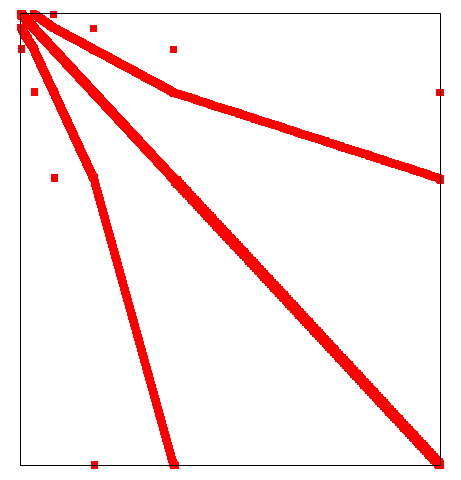
\includegraphics[width=.4\textwidth]{graph/step-2-sparsity-1}
    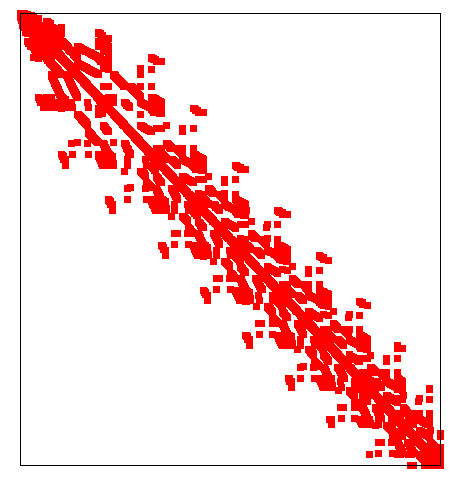
\includegraphics[width=.4\textwidth]{graph/step-2-sparsity-2}
  \end{center}
  \begin{itemize}
  \item All matrices for the same finite element space have the same sparsity pattern
  \end{itemize}
\end{frame}

\subsection{Problems}
\begin{frame}
  \frametitle{Exercises: finite element spaces and sparsity}
  {\footnotesize{\url{http://www.dealii.org/\dealrelease/doxygen/deal.II/step_2.html}}}
  \begin{itemize}
  \item Additional information:
    \begin{itemize}
    \item \texttt{SparsityPattern::bandwidth()}
    \item \texttt{SparsityPattern::n\_nonzero\_elements()}
    \end{itemize}
  \item Problems: study how these numbers depend on
    \begin{itemize}
    \item finite element degree
    \item mesh refinement
    \item space dimension
    \item Choice of
      \begin{itemize}
      \item \lstinline!FE_Q(k) ! $k=1,2,3$
      \item \lstinline!FE_DGQ(k) ! $k=0,1,2,3$
      \item \lstinline!FE_DGP(k) ! $k=0,1,2,3$
      \item \lstinline!FE_Nedelec(k) ! $k=1,2$
      \end{itemize}
    \end{itemize}
  \end{itemize}
\end{frame}


%%% Local Variables: 
%%% mode: latex
%%% TeX-master: "slides"
%%% End: 
